\chapter*{The AD--AS Model}
\section*{Overview}
To make our analysis more realistic and to introduce inflation into the picture, we now present the AD--AS model in \((Y,\pi)\)-space. Here, the horizontal axis represents real output \(Y\) and the vertical axis represents inflation \(\pi\). In our model:
\begin{itemize}
    \item The \textbf{Aggregate Demand (AD)} curve is downward sloping. A higher inflation rate tends to reduce real balances and dampen consumption and investment, thereby lowering output.
    \item The \textbf{Short-Run Aggregate Supply (SAS)} curve is upward sloping. Due to nominal rigidities—such as sticky wages—higher inflation is associated with higher output in the short run.
    \item The \textbf{Classical Aggregate Supply (AS)} curve is vertical. It represents the economy's potential output \(Y^*\), which is determined by real factors like technology and resources. In the long run, inflation does not affect real output.
\end{itemize}
The figure below shows a typical AD--AS diagram with these characteristics. In this example, we set the potential output at \(Y^*=5\) and assume an equilibrium at \(E=(5,3)\).
\begin{figure}[ht]
    \centering
    \begin{tikzpicture}[scale=1.0]
        \draw[->] (0,0) -- (10,0) node[right] {\(Y\) (Output)};
        \draw[->] (0,0) -- (0,7) node[above] {\(\pi\) (Inflation)};
        \draw[thick] (5,0) -- (5,7) node[above left] {AS};
        \draw[thick,red] (1,1) -- (9,5) node[right] {SAS};
        \draw[thick,blue] (1,5) -- (9,1) node[right] {AD};
        \draw[dotted] (5,0) -- (5,3) -- (0,3);
        \fill (5,3) circle (2pt);
        \node[xshift=0.25cm, yshift=0.4cm] at (5,3) {\(E\)};
    \end{tikzpicture}
    \caption{AD--AS diagram in \((Y,\pi)\)-space. The downward-sloping AD (blue) and upward-sloping SAS (red) curves intersect at \(E=(5,3)\). The vertical AS curve (black) shows potential output \(Y^*=5\).}
\end{figure}

\bigskip

\noindent \textbf{Discussion:}
\begin{itemize}
    \item In the short run, if an aggregate demand shock occurs (e.g., expansionary fiscal policy), the AD curve shifts. Depending on the monetary policy response, the Central Bank may allow inflation to change.
    \item If the economy is operating below potential, downward pressure on wages may shift SAS rightward, eventually restoring equilibrium at the potential output (AS).
    \item The Taylor rule and the Central Bank's reaction function (adjusting interest rates to target a specific inflation rate) help determine the slope of the AD curve.
\end{itemize}

\section*{AD--AS Equilibrium and the Impact of Shocks}
\subsection*{Baseline Equilibrium}
In the long-run equilibrium the economy's actual output equals its potential output. For example, consider the following baseline curves in \((Y,\pi)\)-space:
\begin{itemize}
    \item \(\textbf{AD:}\) \(\pi = -0.5\,Y + 5.5\)
    \item \(\textbf{SAS:}\) \(\pi = 0.5\,Y + 0.5\)
    \item \(\textbf{AS:}\) Vertical line at \(Y^*=5\)
\end{itemize}
These curves intersect at the equilibrium point \(E_0=(5,3)\).
\begin{figure}[ht]
    \centering
    \begin{tikzpicture}[scale=1.0]
        \draw[->] (0,0) -- (10,0) node[right] {\(Y\) (Output)};
        \draw[->] (0,0) -- (0,7) node[above] {\(\pi\) (Inflation)};
        \draw[thick] (5,0) -- (5,7) node[above left] {AS};
        \draw[thick,red] (1,1) -- (9,5) node[right] {SAS};
        \draw[thick,blue] (1,5) -- (9,1) node[right] {AD};
        \draw[dotted] (5,0) -- (5,3) -- (0,3);
        \fill (5,3) circle (2pt);
        \node[xshift=0.25cm, yshift=0.4cm] at (5,3) {\(E_0\)};
    \end{tikzpicture}
    \caption{Baseline AD--AS diagram in \((Y,\pi)\)-space with \(E_0=(5,3)\) and potential output \(Y^*=5\).}
\end{figure}

\subsection*{Analysis of Shocks:}
Suppose the economy is hit by a severe shock---such as a major natural disaster---that:
\begin{itemize}
    \item \textbf{Negatively affects aggregate supply (AS):} The destruction of capital assets reduces production possibilities. Although some capital can be rebuilt over several years, adverse demographic impacts (e.g., loss of human capital) may make part of this shock permanent. Graphically, this shifts the short‑run aggregate supply (SAS) curve upward (reflecting higher production costs) and the classical aggregate supply (AS) curve leftward (reflecting a lower potential output).
    \item \textbf{Negatively affects aggregate demand (AD):} Losses in income and consumer confidence may also reduce spending. However, some types of spending may simply be re‐allocated (for example, from discretionary spending to rebuilding), so the AD shock may be more modest.
\end{itemize}
Below is a diagram illustrating a new, post-shock equilibrium. In our example, we assume:
\begin{itemize}
    \item The new potential output falls from \(Y^*=5\) to \(Y^*=4.5\) (AS shifts left).
    \item The SAS curve shifts upward by 1 unit (reflecting cost-push effects), so that the new SAS is given by: 
    \[
    \pi = 0.5\,Y + 1.5.
    \]
    \item The AD curve shifts left modestly, to, for example: 
    \[
    \pi = -0.5\,Y + 5.3.
    \]
\end{itemize}
The new short-run equilibrium \(E'\) is determined by the intersection of the new SAS and AD curves. Solving
\[
0.5\,Y + 1.5 = -0.5\,Y + 5.3,
\]
we find:
\[
Y = 3.8 \quad \text{and} \quad \pi = 0.5(3.8) + 1.5 \approx 3.4.
\]
Thus, \(E'=(3.8,3.4)\).
\begin{figure}[ht]
    \centering
    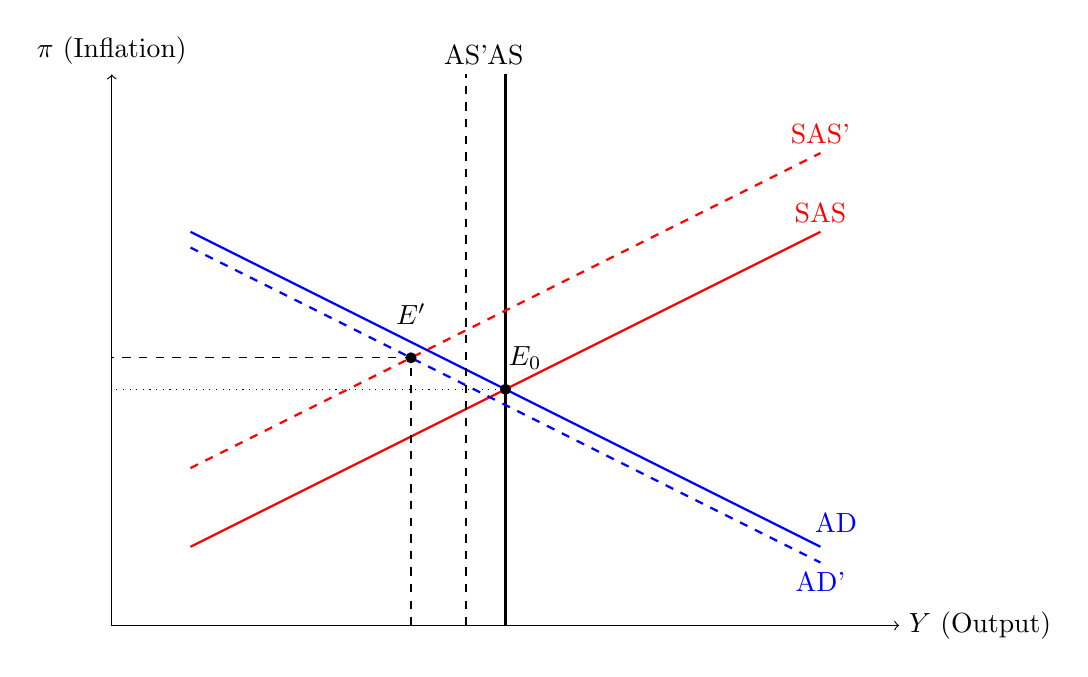
\begin{tikzpicture}[scale=1.0]
        \draw[->] (0,0) -- (10,0) node[right] {\(Y\) (Output)};
        \draw[->] (0,0) -- (0,7) node[above] {\(\pi\) (Inflation)};
        \draw[thick] (5,0) -- (5,7);
        \node[above] at (5,7) {AS};
        \draw[thick,red] (1,1) -- (9,5);
        \node[red,above] at (9,5) {SAS};
        \draw[thick,blue] (1,5) -- (9,1);
        \node[blue,xshift=0.2cm, yshift=0.3cm] at (9,1) {AD};
        \draw[dotted] (5,0) -- (5,3) -- (0,3);
        \fill (5,3) circle (2pt);
        \node[xshift=0.25cm, yshift=0.4cm] at (5,3) {\(E_0\)};
        \draw[thick,dashed] (4.5,0) -- (4.5,7);
        \node[above] at (4.5,7) {AS'};
        \draw[thick,red,dashed] (1,2) -- (9,6);
        \node[red,above] at (9,6) {SAS'};
        \draw[thick,blue,dashed] (1,4.8) -- (9,0.8);
        \node[blue,below] at (9,0.8) {AD'};
        \draw[dotted,dashed] (3.8,0) -- (3.8,3.4) -- (0,3.4);
        \fill (3.8,3.4) circle (2pt);
        \node[above=0.3cm] at (3.8,3.4) {\(E'\)};
    \end{tikzpicture}
    \caption{Updated AD--AS diagram with dashed post-shock curves and non-overlapping labels. 
    Baseline curves (solid) intersect at \(E_0\); new curves (dashed) intersect at \(E'\).}
\end{figure}

\subsection*{Interpretation of the Shocks}
\begin{itemize}
    \item \textbf{Aggregate Supply Shock:}  
    The disaster reduces the economy’s production capacity. The short-run aggregate supply (SAS) curve shifts upward due to higher costs, while the long-run (classical) aggregate supply (AS) shifts left, indicating a lower potential output. Although some capital can be rebuilt over time, adverse demographic effects mean that a portion of the shock is permanent.
    \item \textbf{Aggregate Demand Shock:}  
    The loss of income and confidence tends to reduce consumption and investment, shifting the aggregate demand (AD) curve leftward. However, some planned spending may simply be redirected (for example, from leisure to reconstruction), so the demand shock may be relatively modest.
    \item \textbf{New Equilibrium:}  
    The combined effects of the shocks result in a new short-run equilibrium \(E'\) with lower output and a slightly higher inflation rate. In this example, output falls from 5 to about 3.8 and inflation rises from 3 to 3.4, illustrating how negative supply shocks (with some permanent components) can lead to stagflation.
\end{itemize}